%!TEX root =../LibroTipoETSI.tex
\chapter{Introducción}\label{chp-01}


\lettrine[lraise=-0.1, lines=2, loversize=0.2]{E}{n}n las prácticas de laboratorio realizadas por parte de alumnos durante la docencia de los cursos de Robótica del Departamento de Ingeniería de Sistemas y Automática de la Escuela Técnica Superior de Ingeniería de Sevilla, los alumnos tienen como finalidad aprender a controlar un brazo robótico. Con este fin, en una de las prácticas propuestas deben programar el movimiento del brazo robótico disponible en el laboratorio utilizando el programa RobotStudio . El objetivo principal de la práctica consiste en que una pieza sea trasladada por el robot desde un punto inicial hacia una segunda posición siguiendo la trayectoria indicada. Para poder conseguir esto, es habitual que los alumnos necesiten varios intentos de programación y varios ciclos de movimiento del robot para poder obtener un resultado correcto.

El proceso se realiza colocando manualmente la pieza sobre la mesa de trabajo, lo que lleva asociada diferente problemática que puede llegar a interferir en los resultados obtenidos por los alumnos. Por un lado, la precisión es cuestionable, ya que el propio alumno no tiene una referencia sobre la cual poder repetir el proceso de forma eficaz, ya que la referencia empleada suele ser una marca realizada a mano alzada con lapicero sobre la mesa y el posicionamiento lo realiza un alumno. Esto puede influir negativamente dado que la programación establece un punto inicial fijo en unas coordenadas, sin embargo, al tener que repetir varias veces el proceso para modificar la programación de la trayectoria, el punto inicial no se ubica exactamente en las mismas coordenadas, sino que se empiezan a aproximar al punto inicialmente establecido. Por otro lado, al invadir el espacio de trabajo del brazo robótico continuamente se producen riesgos innecesarios impropios de las normas de seguridad en la industria y en el ambiente académico.

Este trabajo es la continuación de Tapia\cite{tapia} e Hinojosa\cite{rea}, que sentaron las bases del proyecto en prototipos teóricos. En esta ocasión, el enfoque es en la implementación sobre los equipos del laboratorio a nivel real. El objetivo es añadir a la práctica una cinta transportadora que controle la posición de la pieza de forma precisa y permita trasladar dicha pieza a través de la cinta. Para que esta cinta pueda ser utilizada por los alumnos, en este trabajo de fin de grado se desarrolla la construcción de un panel de control que permita su manejo. Este panel debe quedar recogido en una caja donde se realicen las conexiones electrónicas y todas las placas empleadas para controlar electrónicamente la cinta para garantizar la seguridad del dispositivo y asegurar que estas conexiones no se modifican accidentalmente en el laboratorio por los alumnos.

Un objetivo secundario establecido en el proyecto consiste en la garantía de reparabilidad, es decir,el sistema debe tener componentes fácilmente sustituibles para facilitar las reparaciones. Ya que, al ser manipulado este dispositivo de forma recurrente por diferentes alumnos, y no profesionales, la probabilidad de avería por uso y desgaste es mayor.

Para poder emplearse en las prácticas, el sistema se diseña para contar con las siguientes características:
\begin{itemize}
	\item Posicionamiento de piezas en la cinta transportadora en medidas de ejes X e Y que el usuario requiera para interactuar con el robot.
	\item Conexión entre Arduino y RobotStudio mediante protocolo TCP/IP para comunicaciones
	\item Funcionamiento sin Arduino mediante señales digitales del robot.
	\item Funcionamiento sin conexión directa entre RobotStudio y Arduino.
\end{itemize}

\section{Modos de funcionamiento}\label{sec-00}

Es necesario establecer diferentes modos de funcionamiento para el dispositivo dado que todas las funciones especificadas no pueden cumplirse al mismo tiempo porque existirían conflictos entre ellas. Es por ello por lo que el sistema debe tener ciertos modos de funcionamiento que se determinan en función del uso que el estudiante necesite.

Para poder organizar los modos de funcionamiento, la primera consideración es determinar qué dispositivo gobierna el sistema o  establecer el dispositivo máster. Pueden existir dos casos, en uno,  el máster es la controladora del robot (o RobotStudio durante una simulación), en el otro caso el máster es el panel de control de usuario de la cinta (Arduino o la propia electrónica interna). Respectivamente serán los modos remoto y local.
En ambos modos existen otros dos tipos de uso dado que el microcontrolador presente en el Arduino puede estar funcionando o no, por lo que se deben añadir las dos posibilidades, introduciendo los modos con microcontrolador y sin microcontrolador. 

En total, se cuenta con cuatro modos de funcionamiento que se describen a continuación. 

\subsection{Modo local con microcontrolador}\label{subsec-01}

En este modo, se podrá testear el correcto funcionamiento de la cinta, se puede establecer la posición final de la pieza mediante los mandos en el panel de control.

Las órdenes del sistema están proporcionadas por los periféricos de entrada presentes, es decir, el máster es el panel de control. El microcontrolador es el encargado de gestionar el posicionamiento y mover el motor de la cinta cuando le sea indicado. 

En este caso el brazo robótico no tiene conocimiento previo de la posición de la pieza, por lo que para poder recoger la pieza necesitará información extra. Para ello, si hay disponible la conexión con la controladora del robot, mediante el cable Ethernet, el Arduino comunica mediante conexión TCP/IP la posición de la pieza en los ejes “X” e “Y” además del estado del sensor fotoeléctrico y del sistema.

\subsection{Modo remoto con microcontrolador}\label{subsec-02}

A diferencia del anterior, en este modo se podrá mover la pieza a cualquier punto deseado de la cinta desde RobotStudio sin necesidad de usar el panel de control de la propia cinta.

El gobierno del sistema pasa a ser parte de la controladora del robot, convirtiendo al microcontrolador en esclavo, pasando a ser RobotStudio el máster.

El microcontrolador sigue encargándose del posicionamiento y movimiento del motor, pero las órdenes pasan a ser recibidas mediante conexión TCP/IP, es decir, el microcontrolador, en este caso, sólamente ejecuta las órdenes de movimiento recibidas mediante los comandos introducidos en RobotStudio. Como en el caso anterior, se envía la posición, estado del sistema y del sensor fotoeléctrico mediante conexión TCP/IP a la controladora.

\subsection{Modo local sin microcontrolador}\label{subsec-03}

Este modo puede ser empleado como modo alternativo de funcionamiento en caso de que la placa Arduino falle.

El máster del sistema, al ser el modo local, es el panel de control de la cinta; sin embargo, al no tener el microcontrolador operativo, el posicionamiento deja de funcionar y las funciones del sistema pasan a ser más básicas, pero sigue funcionando el sistema y puede ser controlado.

El movimiento del motor queda a cargo de la electrónica interna del sistema. Para interactuar con el motor y moverlo se realizará mediante los pulsadores de avance y retroceso. El robot queda no comunicado y solo recibe la señal digital del sensor fotoeléctrico.


\subsection{Modo remoto sin microcontrolador}\label{subsec-04}

Es un modo similar al anterior, dado que la electrónica es la encargada de gestionar el movimiento. La interacción con el sistema se produce mediante señales digitales enviadas por el robot en vez de por el panel de usuario de la cinta.

\section{Distribución de los controles}

Para una interacción con el sistema con el usuario se crea una interfaz hombre-máquina que permite cambiar entre los distintos modos de funcionamiento, visualizar información, controlar el sistema en el modo local y realizar paradas de emergencia en caso de ser necesario. Para ello, se prototipa la interfaz mostrada en la figura 
\ref{fig:interfazhmi}, que posteriormente se explicará en profundidad en el diseño de la caja.

En este diseño se observa un LCD que será el principal encargado de mostrar la información relevante al usuario como la posición o el modo en el que se encuentra el sistema. Por otra parte, se cuenta con dos botones y una flecha de selección, que permiten avanzar por los distintos menús y seleccionar las opciones durante el modo local. Además, las flechas serán las responsables del movimiento de la cinta en el modo local sin microcontrolador. También se cuenta con dos interruptores de dos posiciones cada uno, que permiten seleccionar los modos local/remoto y con microcontrolador/sin microcontrolador.

Por último, una seta de emergencia es imprescindible para realizar una parada de emergencia en caso necesario. La seta está situada en un lugar de fácil acceso y que no interfiere en el uso normal del sistema.


\begin{figure}[htbp]
	\centering
	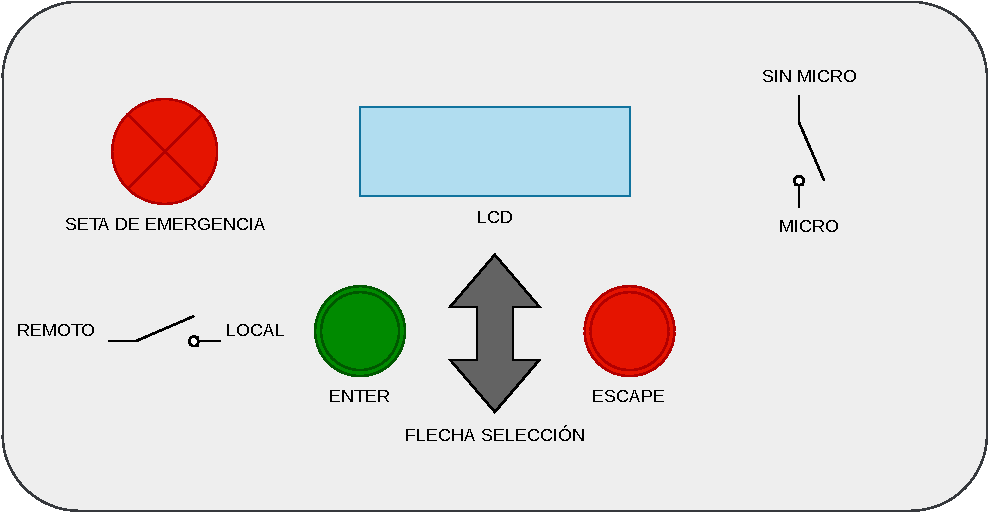
\includegraphics[width=\textwidth]{01-introduccion/HMI.pdf}
	\caption{Interfaz hombre-máquina. Distribución en la tapa.}
	\label{fig:interfazhmi}
	\end{figure}

Además, se debe crear una serie de conexiones que permitan la interacción robot-cinta para el modo remoto sin microcontrolador. Esto se debe realizar mediante un conector que permita acceder a dichos pines de forma sencilla y queden expuestos. Para ello, se introducirá un conector similar a la figura \ref{fig:digitales}. Los pines que debe contener son:
\begin{itemize}
	\item Retroceso.
 	\item Avance.
	\item Local.
	\item Micro.
	\item Emergencia.
  	\item Fotoeléctrico.	
\end{itemize}

\begin{figure}[htbp]
	\centering
	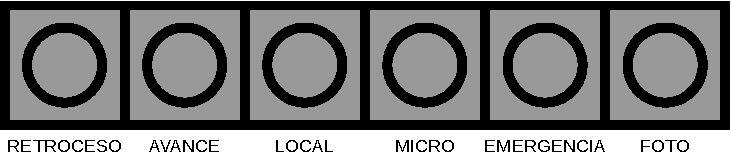
\includegraphics[scale=0.75]{01-introduccion/DIGITALES.pdf}
	\caption{Distribución de conexiones digitales}
	\label{fig:digitales}
	\end{figure}